\documentclass{article}
\usepackage[a4paper,]{geometry}
\usepackage{lmodern}
%\usepackage[export]{adjustbox}
\usepackage[utf8]{inputenc}
\usepackage[T1]{fontenc}
\usepackage{graphicx}
%\usepackage{titlepic}
\usepackage{mathtools}
%\usepackage{amsmath}
%\usepackage{amssymb}
%\usepackage{amsfonts}
\usepackage{wasysym}
%\usepackage{accents}
%\usepackage{esvect}
%\usepackage{subcaption}
\usepackage{multicol}
\usepackage{hyperref}
%\usepackage{enumitem}
\usepackage[makeroom]{cancel}
\usepackage{siunitx}
\usepackage{float}
\usepackage{lipsum}
\usepackage{textcomp}
\usepackage{circuitikz}
\usepackage{placeins}

\sisetup{separate-uncertainty=true}
\linespread{1.3}

% my commands
\newcommand{\E}[1]{\, \mathrm{e}{#1} \, }
\newcommand{\de}{\mathrm{d}}
\newcommand{\pars}{\mathbin{\!/\mkern-5mu/\!}}
\newcommand{\equalexpl}[1]{
	\underset{\substack{\uparrow\\\mathrlap{\text{#1}}}}{=}}

% circuits stuff
\tikzset{
  declare function={% in case of CVS which switches the arguments of atan2
    atan3(\a,\b)=ifthenelse(atan2(0,1)==90, atan2(\a,\b), atan2(\b,\a));},
  kinky cross radius/.initial=+.125cm,
  @kinky cross/.initial=+, kinky crosses/.is choice,
  kinky crosses/left/.style={@kinky cross=-},kinky crosses/right/.style={@kinky cross=+},
  kinky cross/.style args={(#1)--(#2)}{
    to path={
      let \p{@kc@}=($(\tikztotarget)-(\tikztostart)$),
          \n{@kc@}={atan3(\p{@kc@})+180} in
      -- ($(intersection of \tikztostart--{\tikztotarget} and #1--#2)!%
             \pgfkeysvalueof{/tikz/kinky cross radius}!(\tikztostart)$)
      arc [ radius     =\pgfkeysvalueof{/tikz/kinky cross radius},
            start angle=\n{@kc@},
            delta angle=\pgfkeysvalueof{/tikz/@kinky cross}180 ]
      -- (\tikztotarget)}}}



\title{Amplificatore differenziale, Ponte di Wheatstone e Induzione di Faraday}
%\subtitle{Caratteristiche e ponte di Graetz}
\author{Filippo Dal Farra \and Matteo Zandegiacomo Orsolina}
\date{Aprile 2018}

\begin{document}

\maketitle

\newpage

\section{Introduzione}
Questa esperienza è stata divisa in tre parti, nelle quali si sono studiati diversi tipi di circuiti che sfruttano l'uso dei transistor BJT.\\
Nella prima parte si è studiato un amplificatore differenziale a BJT. Questo circuito prevede la possibilità di percepire minime variazioni di tensioni differenziali, sfruttando appunto degli amplificatori che rendono questa differenza più evidente. Lo si è studiato in due configurazioni diverse, nella prima con una resistenza e nella seconda con una sorgente di corrente costante per la polarizzazione dei transistor a cui si sommano le fluttuazioni dovute al segnale in ingresso. Si può così studiare qual è il guadagno differenziale e modo comune del circuito ottenuto dagli ingressi all'uscita.\\

Nella seconda parte dell'esperienza è stato costruito un ponte di Wheatstone. Sono state sfruttate diverse resistenze che ci sono state fornite e un trimmer per bilanciare il ponte. Difatti era nostro interesse trovare la configurazione che meglio riducesse la differenza di tensione all'uscita del ponte. Per studiare ciò si è usato l'amplificatore differenziale precedentemente costruito, in quanto le differenze di tensione risultavano infatti minime e i transistor rispondevano alla necessità di amplificare il segnale per trovare le differenze che altrimenti erano impercettibili dal solo oscilloscopio. \\

Infine, nell'ultima parte dell'esperienza abbiamo riprodotto l'esperimento di Faraday, studiando l'induzione magnetica tra una bobina sorgente (S) e ricevente (R). Così facendo si è in grado di correlare l'elettricità al magnetismo, determinando una relazione tra corrente elettrica e campo magnetico.\\


\section{Materiali e strumenti}
\begin{itemize}
    \item Transistor BJT BC107
    \item Resistenze assortite
    \item Condensatori assortiti
    \item Trimmer
    \item Generatore di funzioni d'onda
    \item Oscilloscopio
    \item Multimetro digitale (DMM)
    \item Due breadboard
    \item Cavi "banana-banana"
    \item Generatore di tensione variabile
    \item Due bobine con N=32 avvolgimenti
    \item Tubo PVC per allineamento bobine
\end{itemize}

\newpage

\section{Procedure di misura}
Innanzitutto si è studiato il comportamento di un amplificatore differenziale a BJT. Per fare ciò è stato costruito il circuito in figura \ref{fig:ampdiff_circ} con $R_C=10\si{\kilo\ohm}$,$R_E=100\si{\ohm}$ e $R_1=10\si{\kilo\ohm}$. Si è fatta scorrere una corrente nominale avente un valore $i_0=0.72\si{\milli\ampere}$ per ciascuno dei transistor e con le resistenze scelte il guadagno differenziale nominale $G_{diff}=50$ e un guadagno modo comune $G_{cm} \approx 0.5$. A questo punto si è potuto procedere con le misure, effettuate variando i valori della frequenza da $100\si{\hertz}$ a $500\si{\kilo\hertz}$. E' stata poi aggiunta una sorgente di corrente come circuito di polarizzazione come rappresentato nella figura \ref{fig:ampdiff_cc_circ} impostando la corrente precedente agendo sul trimmer. Sono state poi effettuate nuovamente le misure, ancora variando il valore della frequenza. \\

In seguito è stato realizzato il ponte di Wheatstone, sfruttando diverse resistenze che ci sono state fornite: una nominale calibrata $R_R = 1000 \Omega$, un trimmer da $2 \si{\kilo\ohm}$ complessivi e una quarta resistenza $R_x$ di cui si doveva trovare il valore grazie al circuito. Una volta costruito si è tentato di bilanciarlo al meglio, modificando la suddivisione delle resistenze sul trimmer, che sono state in seguito misurate grazie al DMM a meno delle inevitabili resistenze di contatto. A questo punto si è potuto ricavare il valore della resistenza incognita. Conoscendo ciò si è stati in grado di procedere con le misure e in particolare \'e stato studiata la risposta del ponte per variazioni $\delta R_x$ aggiungendo in parallelo resistenze da $R = 100 \si{\kilo\ohm}$, per osservare come si modifica l'equilibrio. Togliendo tutte queste resistenze appena aggiunte si è bilanciato nuovamente il ponte, poiché nel frattempo a causa delle varie sollecitazioni che aveva subito poteva essersi modificata l'uscita. Si è così potuto studiare il comportamento del ponte all'aggiunta di condensatori in parallelo aventi valore $\delta C = 1 \si{\nano\farad}$.\\

Nell'ultima parte dell'esperienza è stata innanzitutto costruita una bobina, da utilizzare assieme alla bobina costruita in una precedente esperienza. Le due bobine sono state realizzate allo stesso modo e sono risultate avere lo stesso numero di avvolgimenti, la stessa sezione e lo stesso materiale. Le due bobine, messe una adiacente all'altra, sono state connesse a due circuiti distinti, posti su due breadboard posizionate a decine di centimetri l'una dall'altra. Una di esse è stata alimentata tramite una resistenza $R_{lim}=47 \si{\ohm}$ dal generatore di funzioni, mentre l'altra forniva l'ingresso all'amplificatore differenziale realizzato in precedenza. Si è studiata quindi l'induzione magnetica tra le bobine al variare della frequenza da $1\si{\kilo\hertz}$ a $200\si{\kilo\hertz}$ e della distanza da $20 \si{\milli\meter}$ a $200 \si{\milli\meter}$. Per tutte le misure è stata in particolare salvata la forma d'onda dell'oscilloscopio per l'utilizzo nell'analisi dati.

\newpage

\section{Analisi dei dati}
L'esperienza \'e stata divisa in 3 parti principali, nella prima \'e stato studiato un'amplificatore differenziale a BJT, nella seconda la sua applicazione al ponte di Wheatstone e nella terza e' stato usato per studiare il fenomeno dell'induzione di Faraday.

\subsection{Amplificatore differenziale}

\begin{figure}[h]
    \centering
    \begin{minipage}{0.49\textwidth}
        \centering
        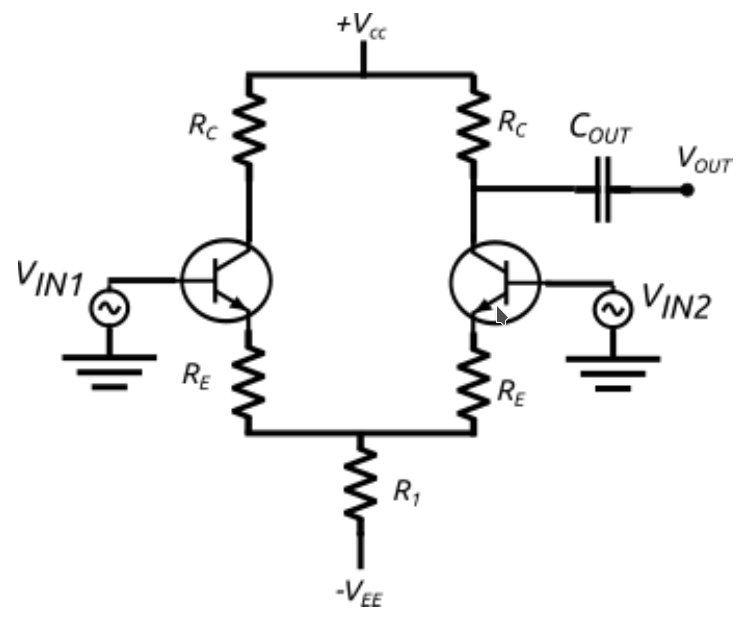
\includegraphics[width=\textwidth]{amp_diff_circ.png} 
        \caption{Amplificatore differenziale senza gene\-ratore corrente costante}
        \label{fig:ampdiff_circ}
    \end{minipage}\hfill
    \begin{minipage}{0.49\textwidth}
        \centering
        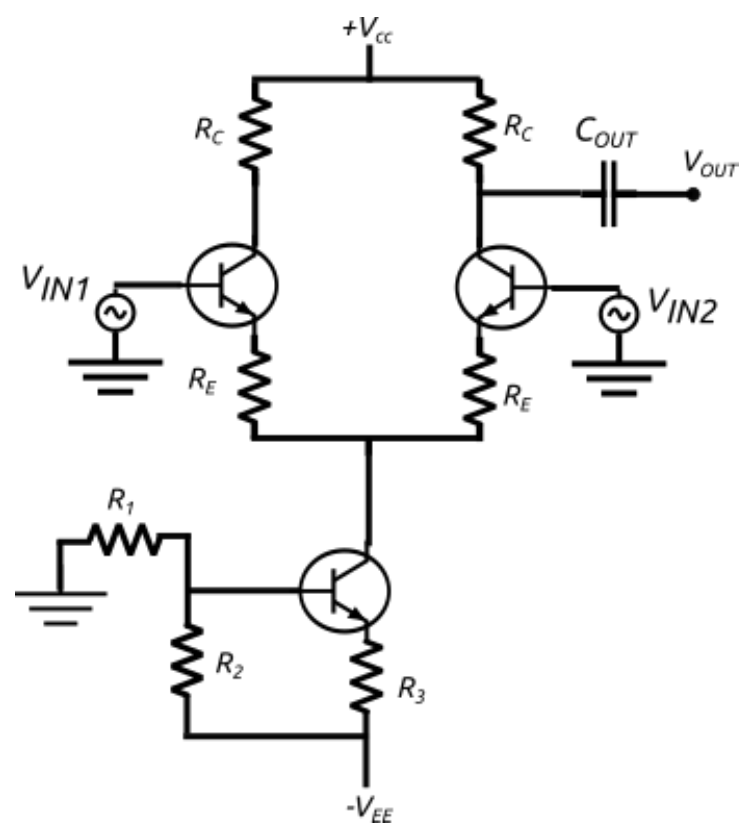
\includegraphics[width=\textwidth]{amp_diff_cc_circ.png} 
        \caption{Amplificatore differenziale con gene\-ratore corrente costante}
        \label{fig:ampdiff_cc_circ}
    \end{minipage}
\end{figure}

Vengono ora mostrati i risultati dei guadagni nelle diverse configurazioni e gli eventuali confronti \ref{fig:gains}.

\begin{figure}[h]
    \centering
    \begin{minipage}{0.5\textwidth}
        \centering
        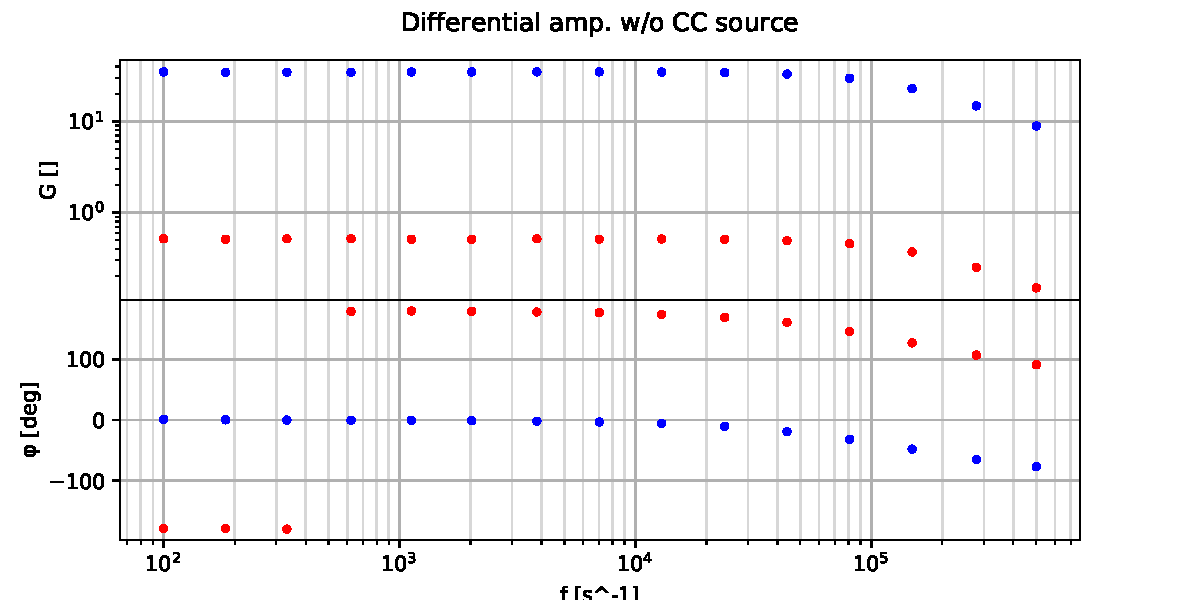
\includegraphics[width=\textwidth]{Figure_1.pdf} 
        %\caption{first figure}
    \end{minipage}\hfill
    \begin{minipage}{0.5\textwidth}
        \centering
        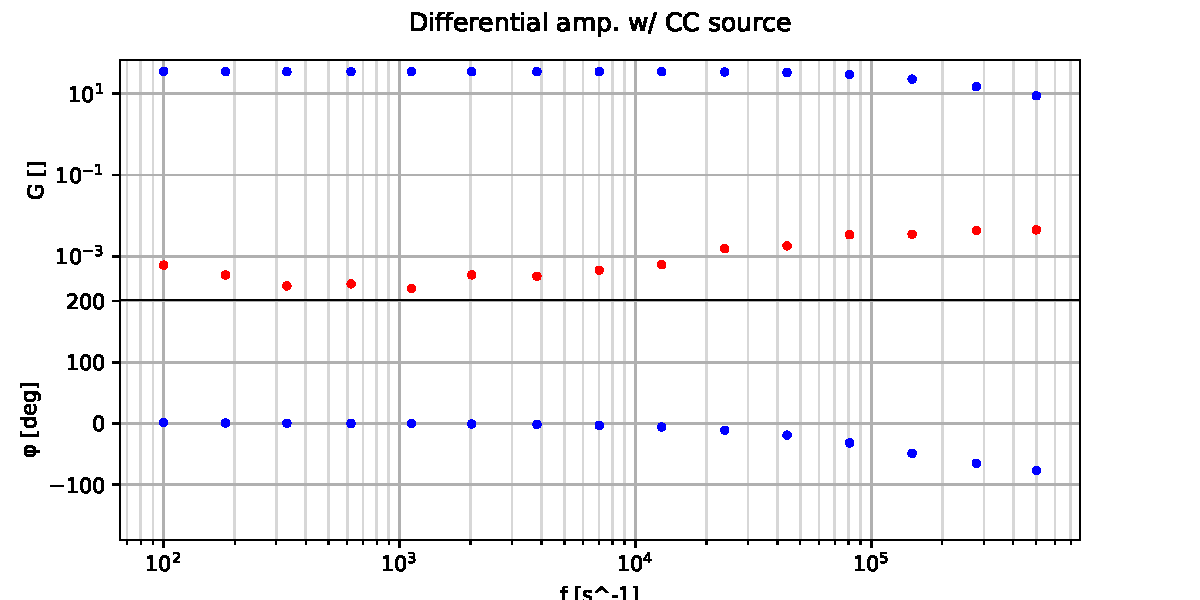
\includegraphics[width=\textwidth]{Figure_2.pdf} 
        %\caption{second figure}
    \end{minipage}
    \\
    \centering
    \begin{minipage}{0.5\textwidth}
        \centering
        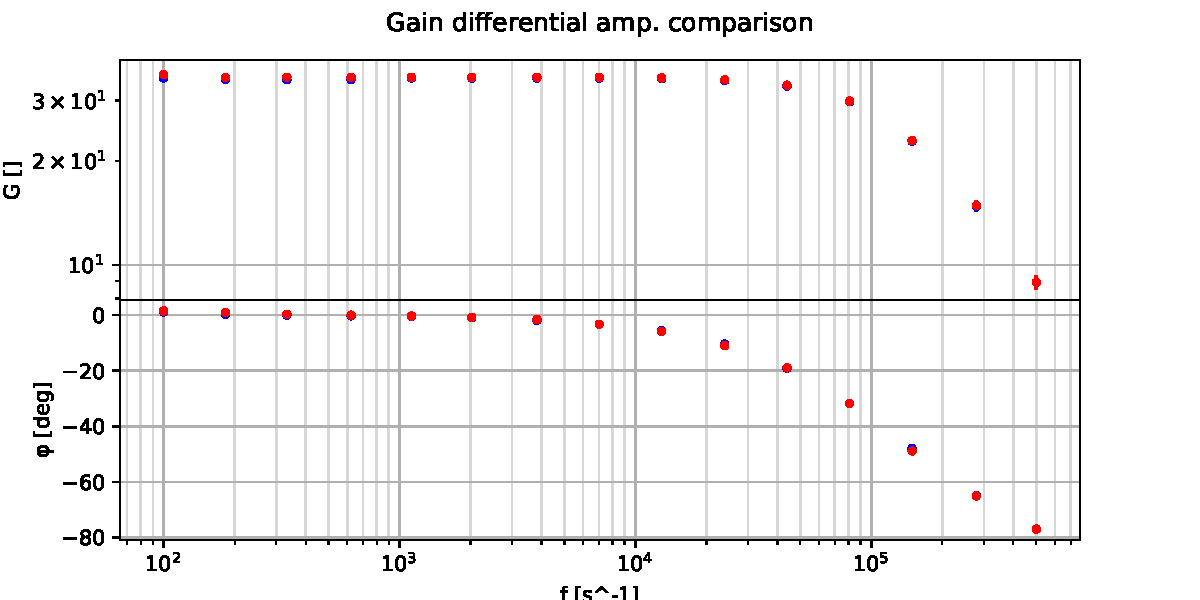
\includegraphics[width=\textwidth]{Figure_3.pdf} 
        %\caption{first figure}
    \end{minipage}\hfill
    \begin{minipage}{0.5\textwidth}
        \centering
        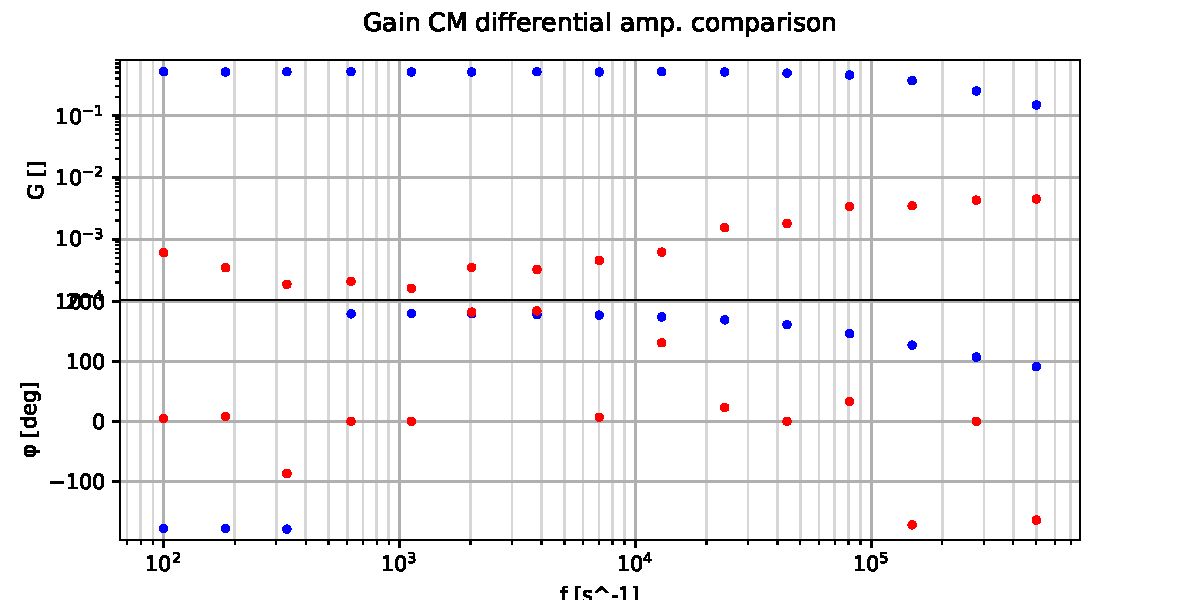
\includegraphics[width=\textwidth]{Figure_4.pdf} 
        %\caption{second figure}
    \end{minipage}
    \caption{Grafici di Bode dei guadagni, spiegazione nel testo.}
    \label{fig:gains}
\end{figure}

Nella riga in alto sono mostrati i guadagni differenziale (in blu) e modo comune (in rosso), senza e con il generatore di corrente costante. Notare innanzitutto che nel diagramma di fase a sinistra il guadagno modo comune passa da $-180 \si{\deg}$ a $+180 \si{\deg}$ per ciclicit\'a degli angoli. Inoltre la fase modo comune con il generatore di corrente non \'e stata misurata per impossibilit\'a di una definizione di essa dato il rumore.\\
Nella riga inferiore sono mostrati i miglioramenti che si ottengono separatamente per i due tipi di guadagno nel caso con (in rosso) e senza (in blu) generatore di corrente costante, come ci aspettiamo il guadagno $G_{diff}$ non risente della circuiteria in pi\'u mentre il modo comune migliora (quindi diminuisce) considerevolmente.\\

Si procede quindi al confronto con un modello di alcune quantit\'a. \\
Il guadagno $G_{diff}$ pu\'o essere calcolato in modo pi\'u preciso con la formula:
\begin{gather}
	G_{diff}=\frac{R_C}{2*(R_E+r_e(i_0))}
\end{gather}
Quindi sapendo che $G_{diff\ max}=35.65$ si pu\'o ottenere il valore di $r_e$:
\begin{gather}
	r_e(i_0)=\frac{R_C-2 G_{diff} R_E}{2 G_{diff}}=40\si{\ohm}
\end{gather}
la quale \'e in linea con quello che ci aspetteremmo per la resistenza di emettitore di un BJT data la corrente $i_0$.

L'impedenza in parallelo al generatore di corrente $Z_S$ pu\'o essere estratta dai dati secondo:
\begin{gather}
	G_{CM}=-\frac{Z_S}{2 R_S} \\
	Z_S(\omega) = -\frac{R_C}{2 G_{CM}}
\end{gather}
e risulta avere un andamento in funzione della frequenza mostrata in figura \ref{fig:zs}.
\begin{figure}[h]
	\centering
    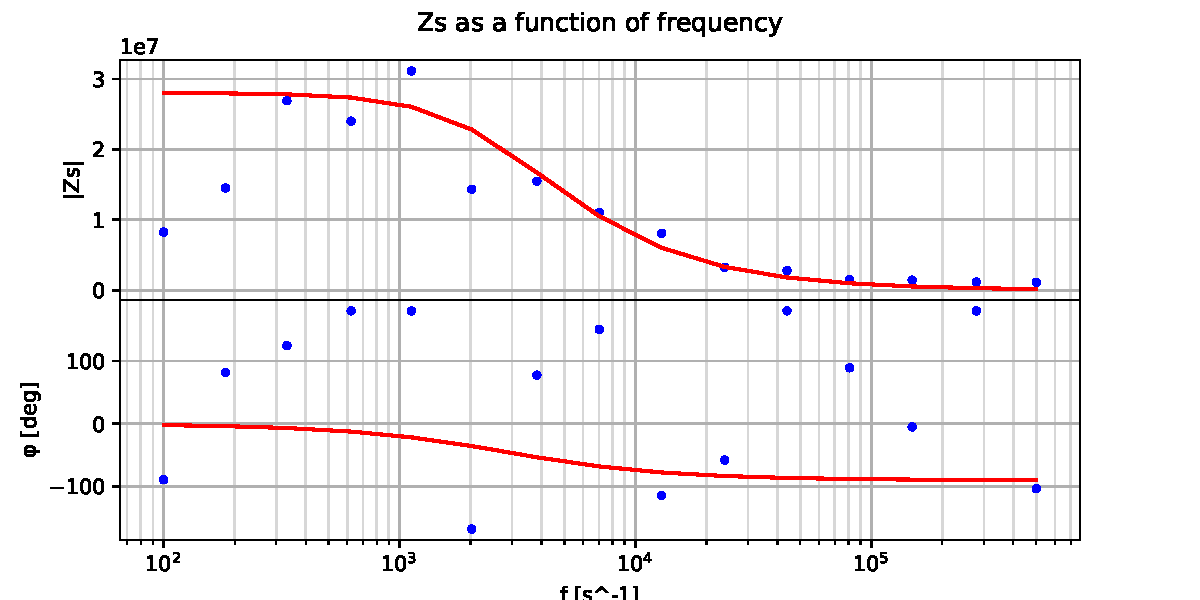
\includegraphics[width=\textwidth]{Figure_5.pdf}
    \label{fig:zs}
    \caption{Andamento di $Z_S$ in funzione della frequenza.}
\end{figure}
Nuovamente la fase misurata di $Z_S$ non \'e affidabile per via del rumore nella misurazione della fase di $G_{CM}$, tuttavia il modulo (in blu) segue l'andamento aspettato superati i $30\si{\kilo\hertz}$ scendendo a $0\si{\ohm}$ il quale \'e compatibile con l'impedenza di un condensatore da $2\si{\pico\farad}$ in parallelo ad una resistenza da $28\si{\mega\ohm}$ mostrati in rosso nella figura entrambi nel range di valori che caratterizzano la giunzione PN del transistor.

\begin{figure}[h]
    \begin{center}
    \begin{circuitikz} []
    \draw
        (0,2) to [sV,l_=$V_{IN} G_{diff}$] (0,0)
        (0,0) to (5,0)
        (0,2) to [R,l=$R_C$] (2,2) 
        (2,2) to [C,l=$C_{out}$] (3,2)
        (3,2) to [C,l_=$C_{osc}$] (3,0)
        (4,2) to [R,l=$R_{osc}$] (4,0)
        (2,2) to (5,2)
        (5,2) to [open, *-*] (5,0);
    \end{circuitikz}
    \caption{Modello $G_{diff}$ misurata.}
    \label{fig:Gdiffmodel}
    \end{center}
\end{figure}

La funzione di trasferimento per il guadagno differenziale tenuto conto del circuito di misura misurato \ref{fig:Gdiffmodel} \'e:
\begin{gather}
	H=G_{diff} \frac{R_{osc} \pars \frac{1}{j\omega C_{osc}}}{R_{osc} \pars \frac{1}{j\omega C_{osc}} + \frac{1}{j\omega C_{out}} + R_C}
\end{gather}
la quale pu\'o essere confrontata, ponendo i valori ottenuti nelle precedenti esperienze per $C_{osc}=110\si{\pico\farad}$ $R_{osc}=1\si{\mega\ohm}$ e il condensatore $C_{out}=100\si{\nano\farad}$ posto in uscita con i dati sperimentali ottenuti in figura \ref{fig:gain_model}.

\begin{figure}[h]
	\centering
    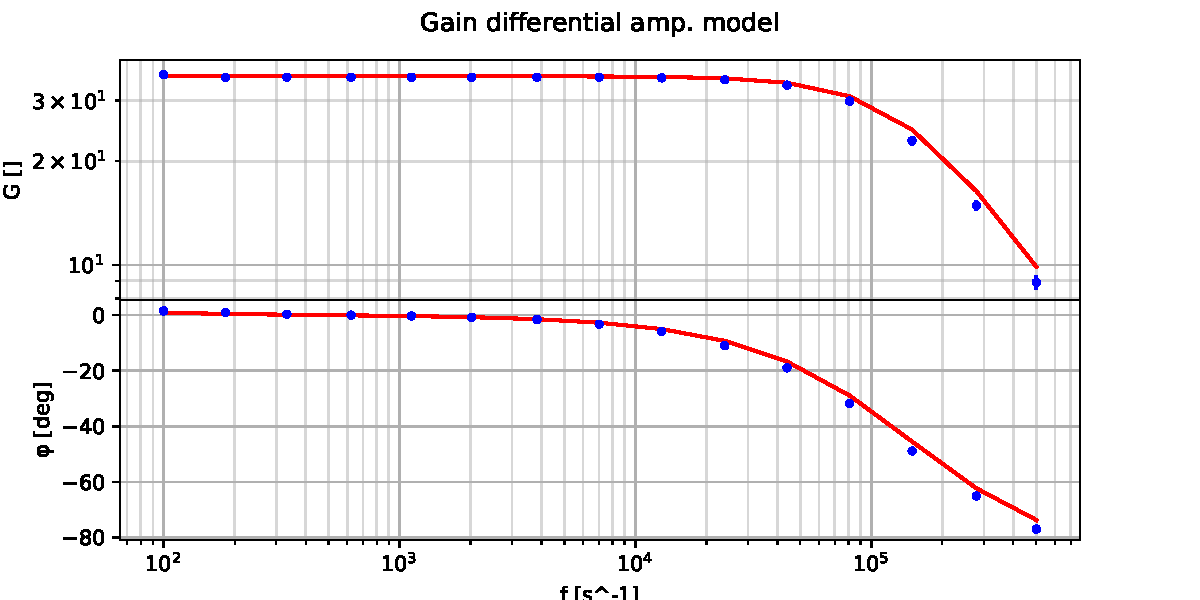
\includegraphics[width=\textwidth]{Figure_6.pdf}
    \label{fig:gain_model}
    \caption{Gain in funzione della frequenza, in blu i punti sperimentali e in rosso la curva del modello.}
\end{figure}
 
 
\newpage
\subsection{Ponte di Wheatstone}
Con il ponte "bilanciato" per il valore $R_x=R_{x0}$ si mostrano in figura \ref{fig:sbil} a titolo di esempio l'output dello "sbilanciamento" che il circuito mostra per diversi valori di $R_{x0}+\delta R_x$ e le misure ripetute sulla stessa configurazione a ponte bilanciato.\\
\begin{figure}[H]
    \centering
    \begin{minipage}{0.49\textwidth}
        \centering
        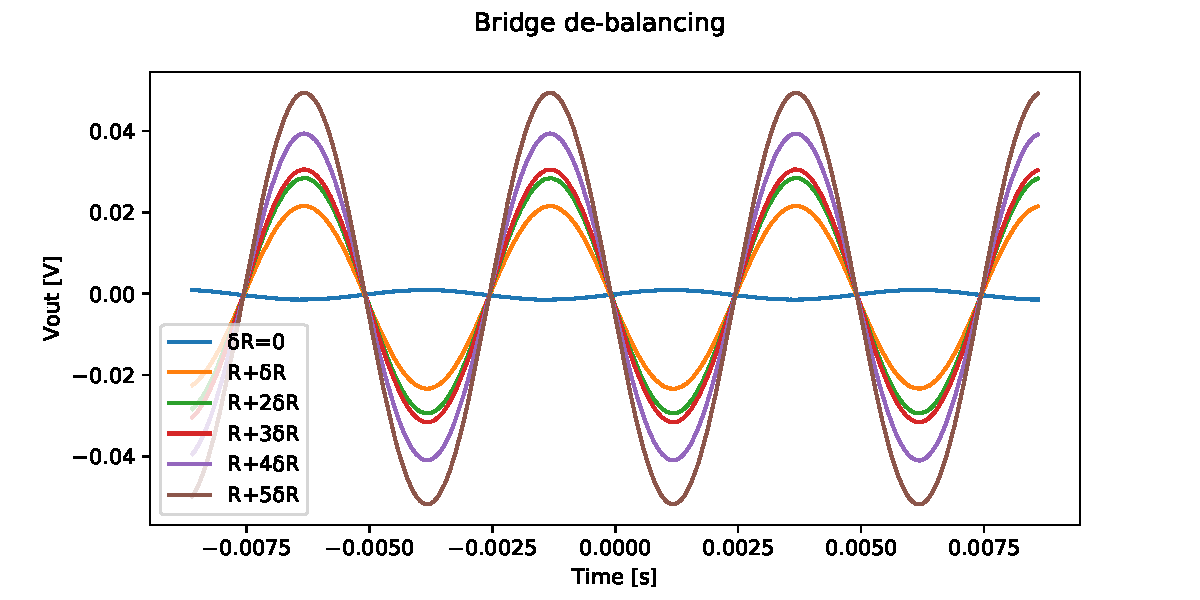
\includegraphics[width=\textwidth]{Figure_12.pdf}
    \end{minipage}\hfill
    \begin{minipage}{0.49\textwidth}
        \centering
        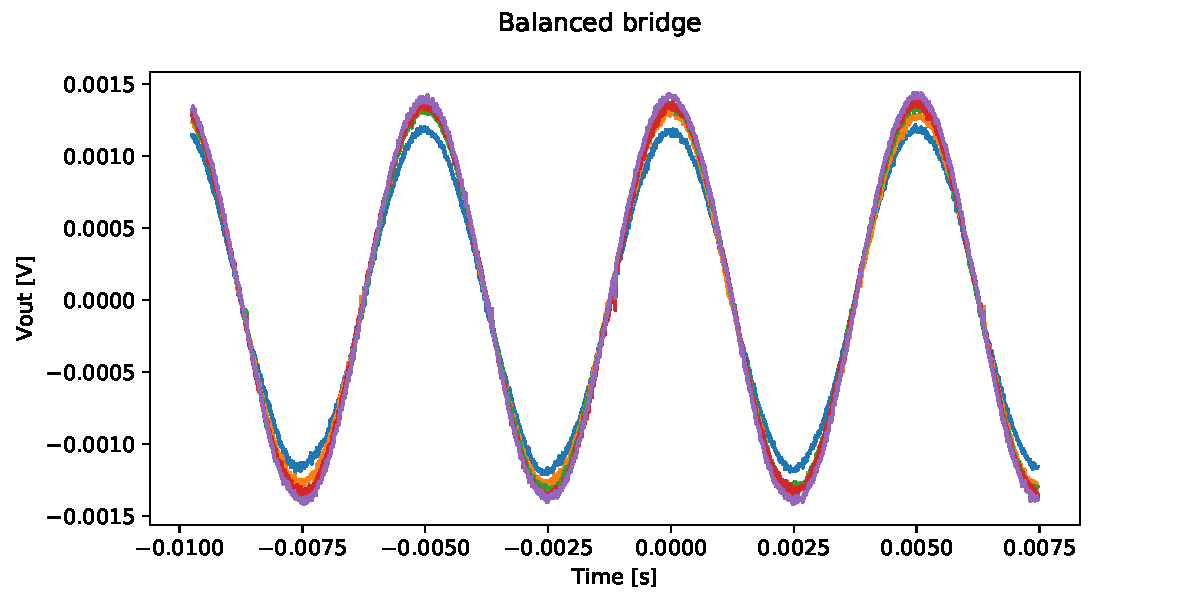
\includegraphics[width=\textwidth]{Figure_18.pdf} 
    \end{minipage}
    \caption{Sbilanciamento allontanandosi da $R_{x0}$ e misure ripetute a ponte bilanciato.}
    \label{fig:sbil}
\end{figure}
Le forme d'onda salvate utilizzando l'oscilloscopio, in modalit\'a 8 averagings, sono state date in input ad una funzione che esegue il fit sinusoidale alla frequenza che era impostata fornendo in output i parametri $A$, $B$ e $V_0$:
\begin{gather}
	V(t)=V_0+A \cos (\omega t)+B \sin (\omega t)
\end{gather}
Tuttavia per l'analisi \'e comodo che il segnale in ingresso sia un coseno puro in modo che il coefficiente $B$ tenda a zero, per fare questo i tempi vengono quindi traslati di un fattore comune sia in ingresso che in uscita partendo da un fit preliminare eseguito sull'ingresso:
\begin{gather}
	\phi=-\arctan (B/A) \\
	t_0=-\frac{\phi}{\omega} \\
	t \rightarrow t-t_0
\end{gather}
I coefficienti $A$ e $B$ possono essere riassunti da un unico numero immaginario trascurando il bias DC $V_0$ in modo che:
\begin{gather}
	V_{in}(t)=V_{0\ in}+V_{in}\cos (\omega t) \\
	V_{out}(t)=V_{0\ out}+A\cos (\omega t)+B\sin (\omega t)= V_{0\ out}+C \cos (\omega t+\phi) =\\
	\nonumber V_{0\ out}+C\cos (\phi)\cos (\omega t) -C \sin (\phi) \sin (\omega t) \\
	\mathbf{Re}[V_{out}]=A=C\cos (\phi) \\
	\mathbf{Im}[V_{out}]=-B=-C\sin (\phi) \\
	V_{out}=A-jB
\end{gather}
Quindi per ogni misurazione effettuata si ottengono due coppie di coefficienti $A$ $B$, una per l'ingresso e una per l'uscita.
Sulle misure ripetute nelle stesse condizioni (5 nel nostro caso) viene eseguita la media aritmetica dei valori e presa come incertezza la deviazione standard diviso $\sqrt{5}$.\\
Vengono quindi mostrati in figura \ref{fig:complan} gli effetti delle piccole variazioni di impedenza sulla risposta del ponte di misura.
\begin{figure}[h]
	\centering
    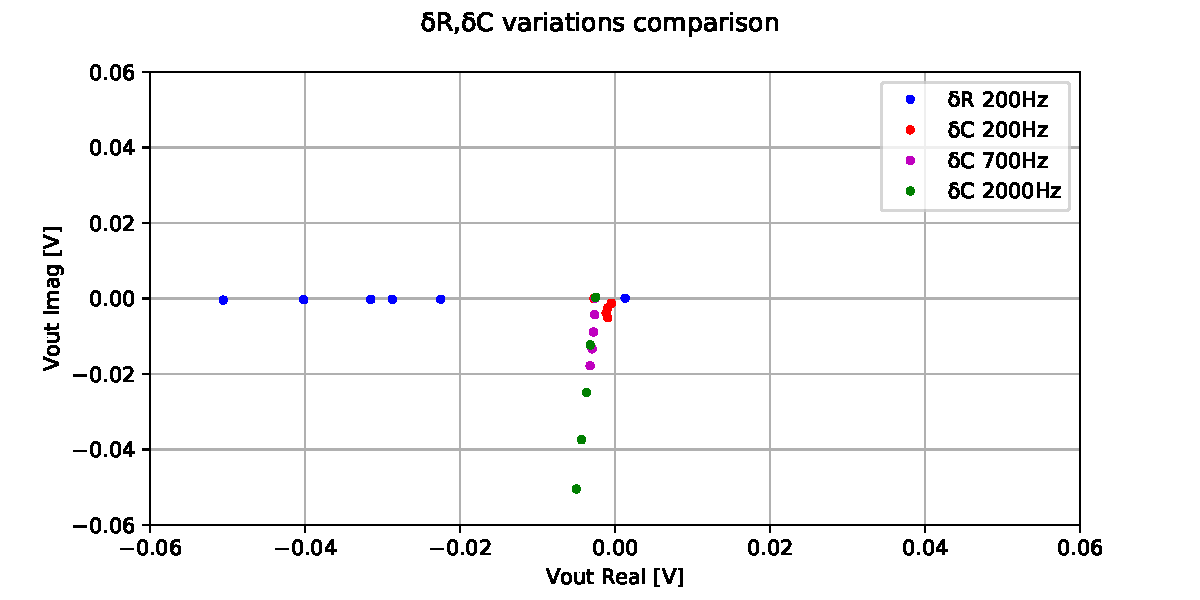
\includegraphics[width=\textwidth]{Figure_7.pdf}
    
    \caption{Plot di $V_{out}$ misurata sul piano immaginario.}
    \label{fig:complan}
\end{figure}
Si vede dalla figura come l'aggiunta di una componente puramente passiva non modifica sensibilmente la fase in uscita mentre se possiede componenti reattive l'effetto su $V_{out}$ \'e quello di uno sfasamento rappresentato da componenti immaginarie prominenti rispetto a quelle reali.\\
Per discriminare ulteriormente gli effetti si procede ad analizzare i vari casi separatamente.
\begin{figure}[h]
    \centering
    \begin{minipage}{0.5\textwidth}
        \centering
        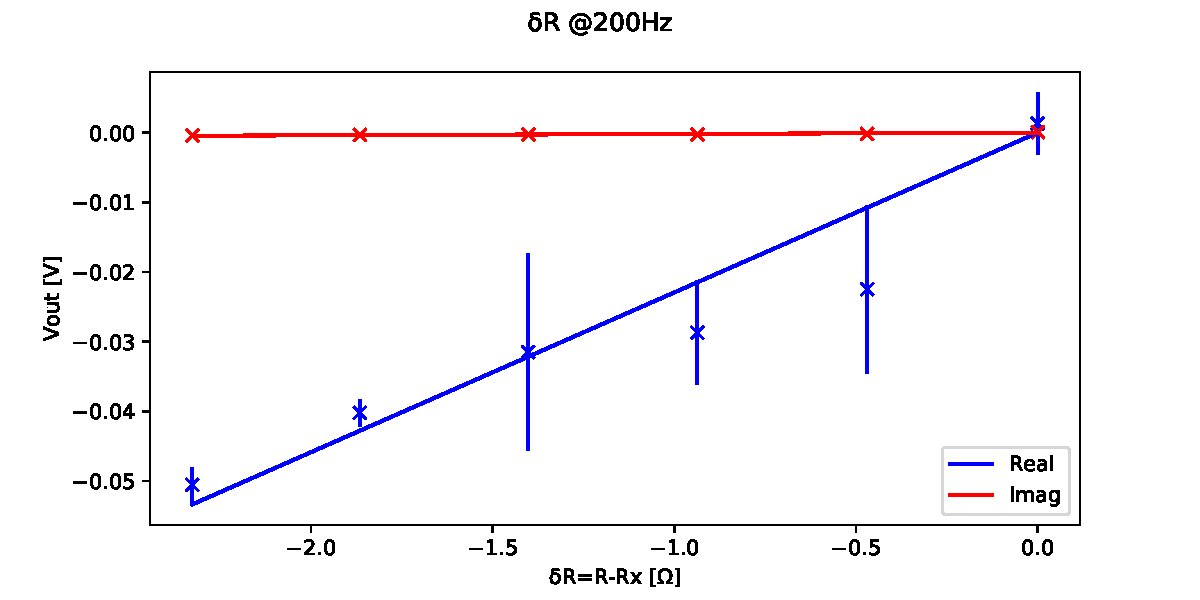
\includegraphics[width=\textwidth]{Figure_8.pdf} 
        %\caption{first figure}
    \end{minipage}\hfill
    \begin{minipage}{0.5\textwidth}
        \centering
        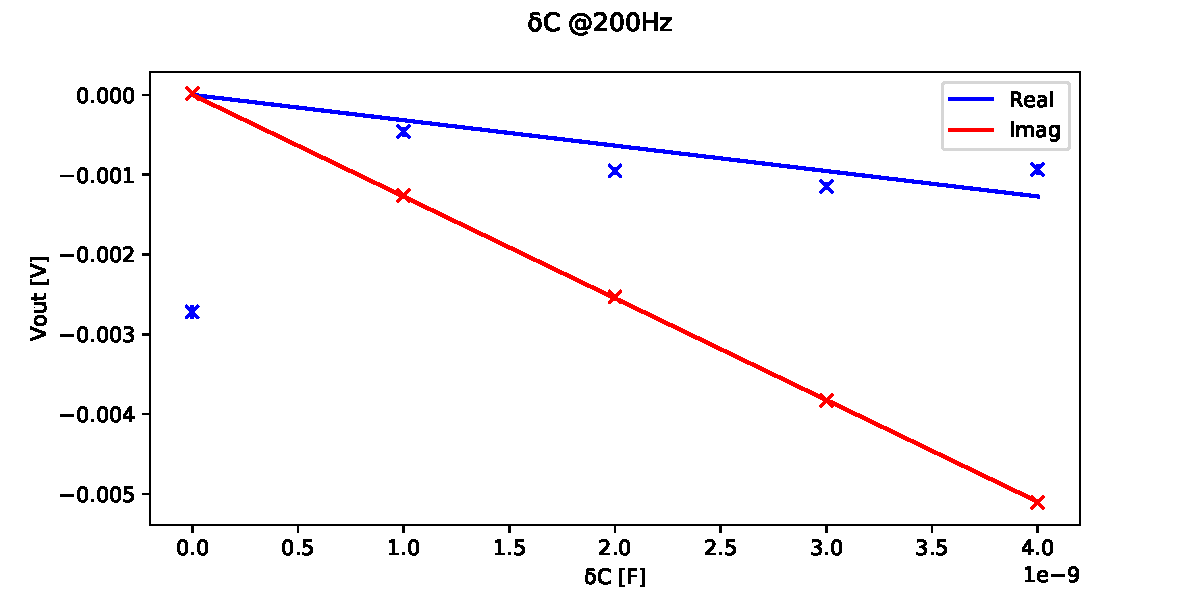
\includegraphics[width=\textwidth]{Figure_9.pdf} 
        %\caption{second figure}
    \end{minipage}
    \\
    \centering
    \begin{minipage}{0.5\textwidth}
        \centering
        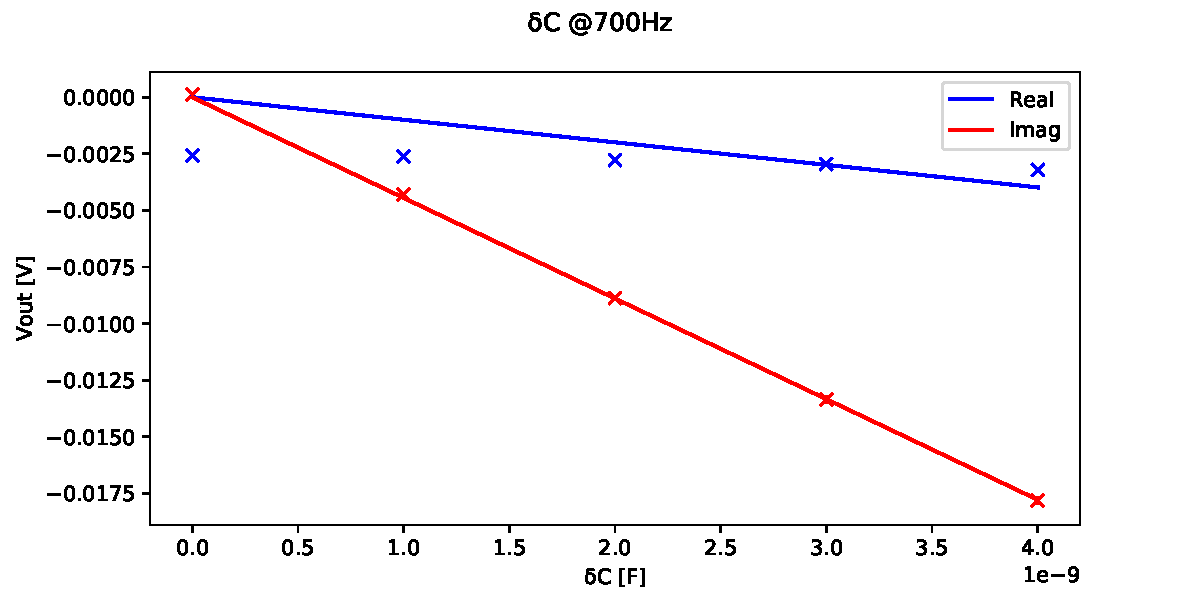
\includegraphics[width=\textwidth]{Figure_10.pdf} 
        %\caption{first figure}
    \end{minipage}\hfill
    \begin{minipage}{0.5\textwidth}
        \centering
        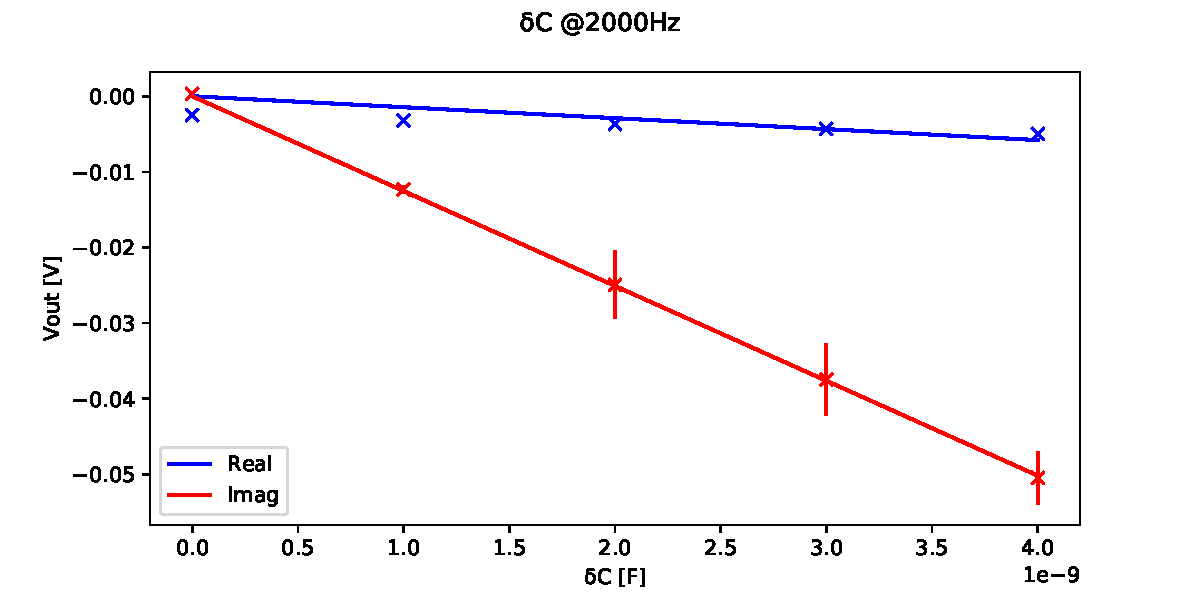
\includegraphics[width=\textwidth]{Figure_11.pdf} 
        %\caption{second figure}
    \end{minipage}
    \caption{$V_{out}$ in funzione di $\delta Z_x$}
    \label{fig:deltaz}
\end{figure}
Per ogni set di dati si procede ad effettuare una regressione lineare del tipo:
\begin{gather}
	\mathbf{Re}[V_{out}]=B \delta R_x \qquad \text{or}\\
	\mathbf{Im}[V_{out}]=B \delta C_x
\end{gather}
E si ottengono i risultati seguenti:
\begin{gather}
	\frac{\partial \mathbf{Re}[V_{out}]}{\partial \delta R_x} = 0.022934+/-0.000013 \ \si{\ampere} \\
	\frac{\partial \mathbf{Im}[V_{out}]}{\partial \delta C_x} = (-1.274+/-0.004)\E{6} \ \si{\volt\per\farad} \ @ \  200 \ \si{\hertz}\\
	\frac{\partial \mathbf{Im}[V_{out}]}{\partial \delta C_x} = (-4.4456+/-0.0010)\E{6} \ \si{\volt\per\farad} \ @ \  700 \ \si{\hertz}\\
	\frac{\partial \mathbf{Im}[V_{out}]}{\partial \delta C_x} = (-1.25414+/-0.00029)\E{7} \ \si{\volt\per\farad} \ @ \  2000 \ \si{\hertz}
\end{gather}
Tuttavia i $\chi^2_{red}$ sono rispettivamente $3343$, $0.9$, $790$ e $22981$ i quali non mostrano compatibilit\'a con la teoria se non nel secondo caso, si procede quindi ad assumere una sottostima delle incertezze che vengono quindi ampliate di conseguenza imponendo $\chi^2_{red}=1$ come \'e gi\'a stato mostrato nei plot in figura \ref{fig:deltaz}. Si ottengono quindi i valori (precedenti) con le nuove incertezze:
\begin{gather}
	\frac{\partial \mathbf{Re}[V_{out}]}{\partial \delta R_x} = 0.0229+/-0.0007 \ \si{\ampere} \\
	\frac{\partial \mathbf{Im}[V_{out}]}{\partial \delta C_x} = (-1.27+/-0.10)\E{6} \ \si{\volt\per\farad} \ @ \  200 \ \si{\hertz}\\
	\frac{\partial \mathbf{Im}[V_{out}]}{\partial \delta C_x} = (-4.4456+/-0.0010)\E{6} \ \si{\volt\per\farad} \ @ \  700 \ \si{\hertz}\\
	\frac{\partial \mathbf{Im}[V_{out}]}{\partial \delta C_x} = (-1.25+/-0.04)\E{7} \ \si{\volt\per\farad} \ @ \  2000 \ \si{\hertz}
\end{gather}

Si procede ora ad effettuare il calcolo della sensibilit\'a del circuito, ovvero la minima variazione di $\delta Z_x$ che esso \'e in grado di risolvere. \\
\begin{gather}
	\sigma_{\delta R} = \frac{ \sigma[\mathbf{Re}[V_{out}]] }{ \frac{\partial \mathbf{Re}[V_{out}]}{\partial \delta R_x}} = 0.6\ \si{\ohm} \\
	\sigma_{\delta C}=\frac{\sigma [\mathbf{Im}[V_{out}]]}{\frac{\partial \mathbf{Im}[V_{out}]}{\partial \delta C_x}} = 1\E{-11} \ \si{\farad} \ @ \  200 \ \si{\hertz} \\
	\sigma_{\delta C}= 2\E{-11} \ \si{\farad} \ @ \  700 \ \si{\hertz} \\
	\sigma_{\delta C}= 1.3\E{-11} \ \si{\farad} \ @ \  2000 \ \si{\hertz}
\end{gather}

\newpage
\subsection{Induzione di Faraday}
Per l'acquisizione delle forme d'onda vengono prese le medesime accortezze della sezione precedente.
\begin{figure}[h]
    \centering
    \begin{minipage}{0.5\textwidth}
        \centering
        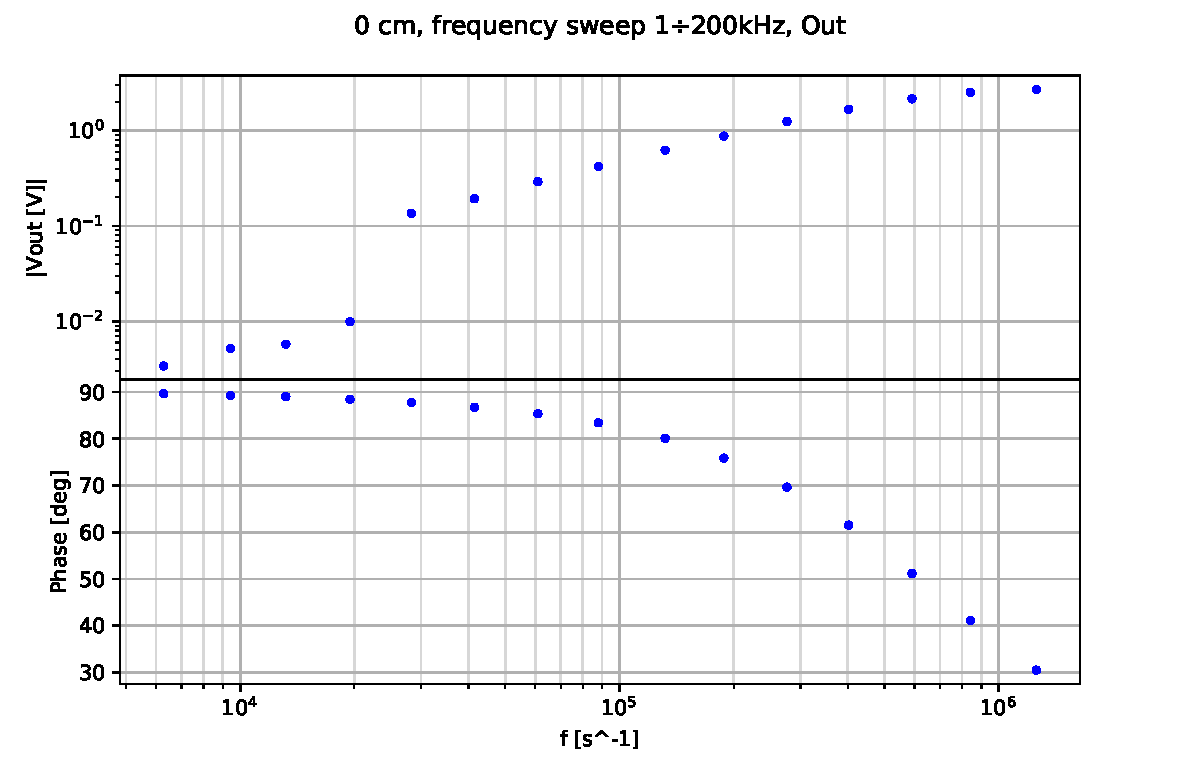
\includegraphics[width=\textwidth]{Figure_13.pdf} 
        %\caption{first figure}
    \end{minipage}\hfill
    \begin{minipage}{0.5\textwidth}
        \centering
        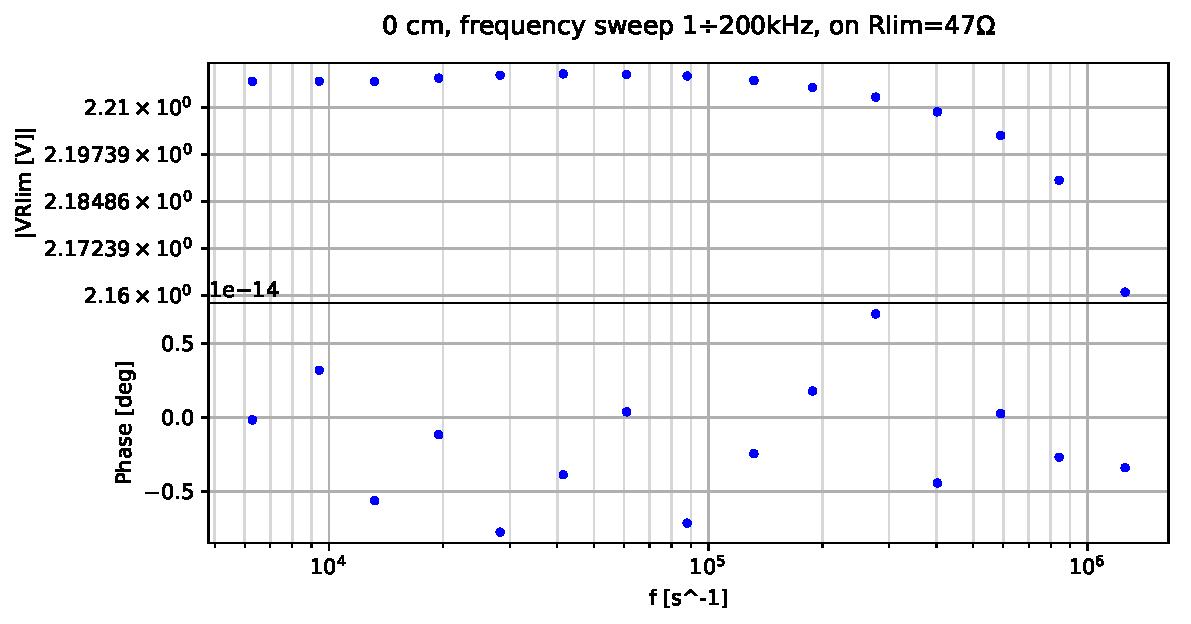
\includegraphics[width=\textwidth]{Figure_14.pdf} 
        %\caption{second figure}
    \end{minipage}
    \caption{Ampiezza dell'induzione e della corrente sulla sorgente al variare della frequenza.}
    \label{fig:induz}
\end{figure}
Dati i plot dei dati raccolti in figura \ref{fig:induz} si pu\'o procedere a calcolare il coefficiente di mutua induzione tra bobina sorgente e ricevente definendo $\epsilon_R$ la f.e.m. ai capi della ricevente in ingresso all'amplificatore e $i_S$ la corrente che scorre nella bobina sorgente misurata sapendo la tensione ai capi di $R_{lim}$:
\begin{gather}
	Z_{eff}(\omega) = \frac{\epsilon_R(\omega)}{i_S(\omega)}= \frac{V_{out}(\omega)}{G_{diff}(\omega) i_S(\omega)} \\
\end{gather}
Supponendo poi che l'accoppiamento sia di tipo induttivo, si pu\'o porre:
\begin{gather}
	Z_{eff}(\omega)=j \omega M_{RS} \\
	M_{RS} = \frac{\epsilon_R(\omega)}{\frac{\partial i_S(\omega)}{\partial t} j} = \frac{\epsilon_R(\omega)}{i_S(\omega) \omega j}
\end{gather}
Viene quindi scelto come valore di $M_{RS}$ la media alle varie frequenze:
\begin{gather}
	M_{RS}= 2.088\E{-6}-j1.049\E{-7}\ \si{\henry} \\
	M_{RS,abs}=2.0916\E{-6}\ \si{\henry} \\
	M_{RS,angle}=-2.8758 \ \si{\deg}
\end{gather}
Come si pu\'o vedere il valore non e' puramente reale come ci si aspetterebbe ma a causa della non nulla resistivit\'a del filo presenta una parte immaginaria, tuttavia la fase risultante \'e talmente prossima a zero che non da un contributo significativo pertanto il risultato \'e compatibile con una misura di induttanza. \\
Viene quindi mostrato in figura \ref{fig:zeff} il confronto dell'impedenza di questa induttanza di accoppiamento con la $Z_{eff}$ misurata cos\'i da verificare che effettivamente il modello valga.
\begin{figure}[h]
	\centering
    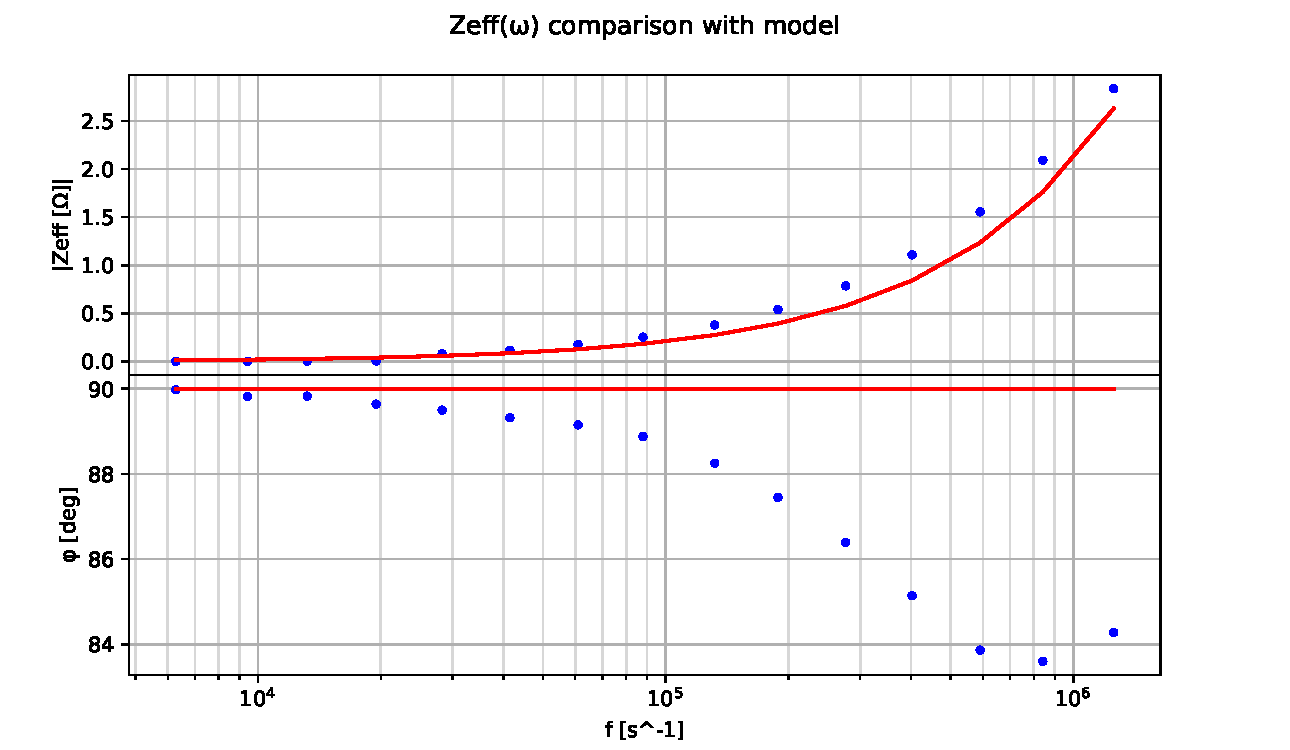
\includegraphics[width=\textwidth]{Figure_15.pdf}
    
    \caption{Confronto tra $Z_{eff}$ in blu e l'impedenza del coefficiente di mutua induzione in rosso.}
    \label{fig:zeff}
\end{figure}
La deviazione della fase, seppur di pochi gradi, pu\'o essere attribuita ad effetti di ordine maggiore qui non presi in considerazione.\\

Si analizza ora l'andamento dell'induzione all'aumentare della distanza, figura \ref{fig:brut}.
\begin{figure}[H]
	\centering
    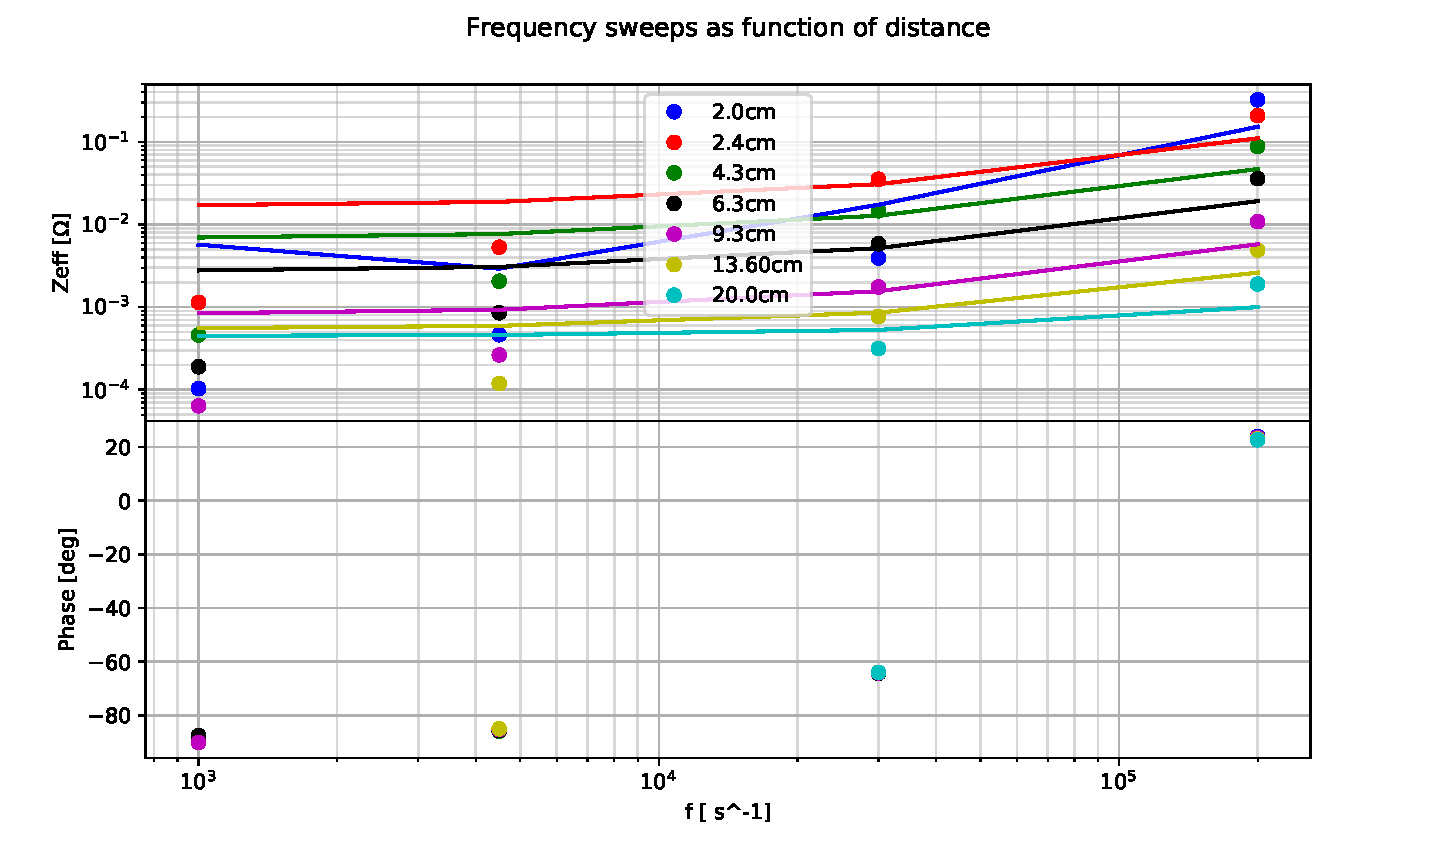
\includegraphics[width=\textwidth]{Figure_16.pdf}
    
    \caption{Confronto a varie distanze in funzione della frequenza.}
    \label{fig:brut}
\end{figure}
L'andamento della fase non \'e quello aspettato e dovrebbe essere indagato pi\'u a fondo con nuovi dati ed un nuovo setup, tuttavia mi aspetto che il modulo aumenti con la frequenza come \'e successo precedentemente.\\
Viene ora scelta la frequenza di $200\ \si{\kilo\hertz}$ per la quale ho dati a tutte le distanze e viene mostrato in figura \ref{fig:r3} il coefficiente di mutua induzione calcolato dalle misure di tensione in entrata ed in uscita comparato all'induzione che un dipolo magnetico esercita su una spira che si muove lungo l'asse di simmetria.\\
\begin{figure}[h]
	\centering
    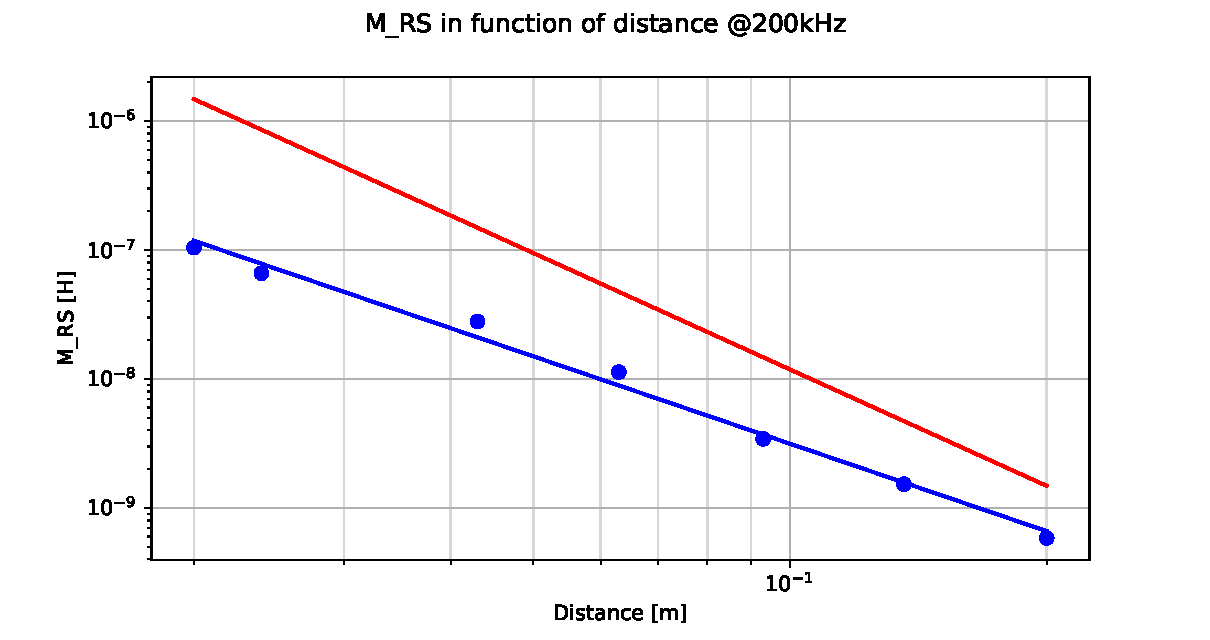
\includegraphics[width=\textwidth]{Figure_17.pdf}
    
    \caption{Mutua induzione in funzione della distanza.}
    \label{fig:r3}
\end{figure}
In rosso \'e mostrato il modello teorico:
\begin{gather}
	r=8.75\ \si{\milli\meter} \\
	\Sigma = \pi r^2 \\
	m_S=N i_S \Sigma \\
	B_{asse}=\frac{\mu_0 2 m_S}{4 \pi d^3} \\
	\Phi_B = N B_{asse} \Sigma \\
	M_{RS} = \frac{\Phi_B}{i_S}
\end{gather}
In blu si mostrano i punti sperimentali assieme alla loro regressione lineare sulla scala logaritmica:
\begin{gather}
	M_{RS,log}=\log (M_{RS}) \qquad d_{log}=\log (d)\\
	M_{RS,log,fit}=A+B d_{log} \\
	M_{RS,fit} = \exp (M_{RS,log,fit}) \\
	A=-24.76 \qquad B=-2.25
\end{gather}
Come si pu\'o vedere non solo i punti sperimentali sono traslati in basso ma il coefficiente $B$ rappresentante l'esponente della distanza \'e diverso da $-3$ come compare nella formula teorica sopra esposta, questo provoca un ulteriore incongruenza. Questo tipo di incongruenze sono dovute al fatto che stiamo usando per il modello l'"approssimazione di dipolo magnetico" la quale \'e valida solamente su grandi distanze mentre a piccole distanze non segue pi\'u una legge di tipo $\propto 1/d^3$. Inoltre la spira ha un certo spessore e parte del flusso entrante al primo giro di essa esce prima di concatenarsi a quelle successive provocando quindi una diminuzione del coefficiente di mutua induzione come mostrato nel grafico. Notare inoltre che all'aumentare della distanza la legge teorica raggiunge la regressione effettuata sui punti sperimentali come ci si aspetta.\\

\newpage

\section{Conclusioni}
L'amplificatore differenziale ci ha permesso di studiare le caratteristiche del ponte di Wheatstone e dell'induzione di Faraday con un'accuratezza che semplicemente non era possibile tramite il solo utilizzo dell'oscilloscopio. Il ponte ha permesso in particolare di misurare minime variazioni di impedenza da un valore nominale e ci\'o \'e di enorme utilit\'a nei circuiti di misura dove si vuole avere una risposta in tensione e fase le quali sono pi\'u facilmente misurabili rispetto all'impedenza. L'esperienza sull'induzione di Faraday permette invece di sondare il limite dell'approssimazione di dipolo magnetico a piccole distanze la quale \'e altrimenti pi\'u che valida per gran parte delle applicazioni che si possono incontrare.

\end{document}

Il valore atteso di $V_{out}$ data la funzione di trasferimento e ci\'o che sappiamo sull'amplificatore differenziale \'e:
\begin{gather}
	V_{out}(\omega)=V_{in}(\omega)\frac{R_R}{(R_{x0}+R_R)^2}\left( \delta R_X - (j \omega R_{x0} \delta C_x) R_{x0} \right) \frac{Z^{AMP}_{IN}}{Z^{AMP}_{IN}+Z^{BRIDGE}_{OUT}} G_{diff}(\omega)
\end{gather}